\documentclass{article}
\usepackage{polski}
\usepackage[utf8]{inputenc}
\usepackage{natbib}
\usepackage{graphicx}
\usepackage{xcolor}
\usepackage{mathtools}
\usepackage{amssymb}
\usepackage[makeroom]{cancel}
\usepackage{hyperref}
\newcommand{\norm}[1]{\left\lVert#1\right\rVert}

% czcionka i marginesy
\usepackage[left=2cm,right=2cm,top=2.54cm,bottom=2.54cm]{geometry}
\usepackage{fontspec}
\setmainfont{Calibri}
%

% Dzielenie sekcji na dwie kolumny
\newenvironment{kol2}{\noindent \begin{minipage}[t]{0.5\linewidth}}{\end{minipage}}

\title{Opracowanie Robotyka}
\author{Jan Bronicki, Mateusz Górka}
\date{}


\begin{document}

\maketitle

\tableofcontents
\newpage
\section{Wykład 1}


\subsection{Warunki, aby macierz była macierzą obrotu}

Aby macierz obrotu {\bf R} była macierzą obrotu musi spełniać warunki:

\begin{itemize}
    \item $R^{T}R=I_{3}$ - macierz musi być ortogonalna
    \item $det R=+1$ - macierz musi być {\bf \it prawoskrętna}
    \item $T$ - (Translacja) - może być dowolna
\end{itemize}

\subsection{Jak sprawdzić prawoskrętność?}

Dla:

\begin{itemize}
    \item $i$ - wersor osi {\bf X}
    \item $j$ - wersor osi {\bf Y}
    \item $k$ - wersor osi {\bf Z}
\end{itemize}

Warunki prawoskrętności:

\Large
$$
	\left\{
	\begin{array}{l}
		j \times i = k \\
		j \times k = i \\
		k \times i = j
	\end{array}
	\right.
$$
\normalsize

{\bf $T$} - (Translacja, czyli przesunięcie) - dowolna.

\subsection{Obroty stanowią grupę}

Obroty stanowią grupę, która jest zbiorem działań, w którym jest zdefiniowany element odwrotny i neutralny:

\begin{itemize}
    \item Element neutralny - $I_{3}$
    \item Element odwrotny - $R^{T}$
\end{itemize}

\newpage

\subsection{Macierze obrotów ZXY}

\Large
$$
    rot \left(z, \alpha\right) = \begin{bmatrix}
        {\color{purple} c_{\alpha}} & {\color{red}-}{\color{blue} s_{\alpha}} & 0 \\[0.3em]
        {\color{blue} s_{\alpha}}   & {\color{purple} c_{\alpha}}             & 0 \\[0.3em]
        0                           & 0                                       & 1
    \end{bmatrix}
$$

$$
    rot \left(x, \beta\right) = \begin{bmatrix}
        1 & 0                          & 0                                      \\[0.3em]
        0 & {\color{purple} c_{\beta}} & {\color{red}-}{\color{blue} s_{\beta}} \\[0.3em]
        0 & {\color{blue} s_{\beta}}   & {\color{purple} c_{\beta}}
    \end{bmatrix}
$$


$$
    rot \left(y, \gamma\right) = \begin{bmatrix}
        {\color{purple} c_{\gamma}}             & 0 & {\color{blue} s_{\gamma}}   \\[0.3em]
        0                                       & 1 & 0                           \\[0.3em]
        {\color{red}-}{\color{blue} s_{\gamma}} & 0 & {\color{purple} c_{\gamma}}
    \end{bmatrix}
$$
\normalsize

\section{Wykład 2}

\subsection{Współrzędne jednorodne, rozszerzenie do 4 wymiarów}

\Large
$$
    p_{0} = R_{0}^{1} \cdot p_{1}
$$

$$
	p_0 = R_0^1 p_1
	, \ \
	R_0^1 =
	\left[ \begin{array}{ccc}
		i_1 i_0	& j_1 i_0	& k_1 i_0	\\
		i_1 j_0	& j_1 j_0	& k_1 j_0	\\
		i_1 k_0	& j_1 k_0	& k_1 k_0	\\
	\end{array} \right]
$$

\normalsize

\begin{itemize}
    \item $p_{0}$ - położenie wektora w układzie "0"
    \item $p_{1}$ - położenie wektora w ukłądzie "1"
    \item $R_{0}^{1}$ - macierz obrotu z położenia "0" do "1"
\end{itemize}

Uwzględniając Translacje:

\Large
$$
    p_{0} = R_{0}^{1} \cdot p_{1} + T_{0}^{1}
$$
\normalsize

$T_{0}^{1}$ - to inaczej odległość pomiędzy początkami układów współrzędnych

Dodajemy czwarty wymiar, aby łatwiej manipulować:
\Large
$$
    \begin{pmatrix}
        p_{0} \\
        1
    \end{pmatrix}
    =
    \begin{bmatrix}
        \begin{array}{c|c}
            R_{0_{3x3}}^{1} & T_{0_{3x1}}^{1} \\[0.3em]
            \hline
            0_{_{1x3}}      & 1
        \end{array}
    \end{bmatrix}
    \begin{pmatrix}
        p_{1} \\
        1
    \end{pmatrix}
$$
\normalsize

\newpage

Przykłady, na macierzach jednorodnych (gdzie $T = \left[0, 0, 0\right]^{T}$):



\Large
$$
    Rot(x, \alpha) =
    \begin{bmatrix}
        \begin{array}{ccc|c}
            1 & 0                           & 0                                       & 0 \\[0.3em]
            0 & {\color{purple} c_{\alpha}} & {\color{red}-}{\color{blue} s_{\alpha}} & 0 \\[0.3em]
            0 & {\color{blue} s_{\alpha}}   & {\color{purple} c_{\alpha}}             & 0 \\[0.3em]
            \hline
            0 & 0                           & 0                                       & 1
        \end{array}
    \end{bmatrix}
$$
\normalsize


\Large
$$
    Rot(y, \beta) =
    \begin{bmatrix}
        \begin{array}{ccc|c}
            {\color{purple} c_{\gamma}}             & 0 & {\color{blue} s_{\gamma}}   & 0 \\[0.3em]
            0                                       & 1 & 0                           & 0 \\[0.3em]
            {\color{red}-}{\color{blue} s_{\gamma}} & 0 & {\color{purple} c_{\gamma}} & 0 \\[0.3em]
            \hline
            0                                       & 0 & 0                           & 1
        \end{array}
    \end{bmatrix}
$$
\normalsize



\Large
$$
    Rot(z, \gamma) =
    \begin{bmatrix}
        \begin{array}{ccc|c}
            {\color{purple} c_{\alpha}} & {\color{red}-}{\color{blue} s_{\alpha}} & 0 & 0 \\[0.3em]
            {\color{blue} s_{\alpha}}   & {\color{purple} c_{\alpha}}             & 0 & 0 \\[0.3em]
            0                           & 0                                       & 1 & 0 \\[0.3em]
            \hline
            0                           & 0                                       & 0 & 1
        \end{array}
    \end{bmatrix}
$$
\normalsize


\newpage

Przykłady Translacji po danych osiach (bez rotacji):


\Large
$$
    Trans(x, a) =
    \begin{bmatrix}
        \begin{array}{ccc|c}
            1 & 0 & 0 & a \\[0.3em]
            0 & 1 & 0 & 0 \\[0.3em]
            0 & 0 & 1 & 0 \\[0.3em]
            \hline
            0 & 0 & 0 & 1
        \end{array}
    \end{bmatrix}
$$
\normalsize


\Large
$$
    Trans(y, b) =
    \begin{bmatrix}
        \begin{array}{ccc|c}
            1 & 0 & 0 & 0 \\[0.3em]
            0 & 1 & 0 & b \\[0.3em]
            0 & 0 & 1 & 0 \\[0.3em]
            \hline
            0 & 0 & 0 & 1
        \end{array}
    \end{bmatrix}
$$
\normalsize



\Large
$$
    Trans(z, c) =
    \begin{bmatrix}
        \begin{array}{ccc|c}
            1 & 0 & 0 & 0 \\[0.3em]
            0 & 1 & 0 & 0 \\[0.3em]
            0 & 0 & 1 & c \\[0.3em]
            \hline
            0 & 0 & 0 & 1
        \end{array}
    \end{bmatrix}
$$
\normalsize


Inna interpolacja:

Gdy $T_{0}^{1} = 0$ układy nie są przesunięte względem siebie, ale są skręcone:
np (gdzie 1, to i-te miejsce):

\Large
$$
    p_{1}=e_{i}=\begin{pmatrix}
        0 \\
        1 \\
        0
    \end{pmatrix}
$$

$$
    \begin{pmatrix}
        p_{0} \\
        1
    \end{pmatrix}
    =
    \begin{bmatrix}
        \begin{array}{c|c}
            R_{0_{3x3}}^{1} & 0 \\[0.3em]
            \hline
            0_{_{1x3}}      & 1
        \end{array}
    \end{bmatrix}
    \begin{pmatrix}
        e_{1} \\
        1
    \end{pmatrix}
$$
\normalsize

\newpage

\subsection{Dzięki współrzędnym jednorodnym operacja rotacji i translacji jest reprezentowana przez jedną macierz}

Ważne:

\begin{itemize}
    \item Rotacje następujące po sobię są mnożeniem następujących macierzy obrotu
    \item Współrzędne jednorodne są grupą nieprzemienną, z działaniem "mnożenie macierzy"
          $$
              K =
              \begin{bmatrix}
                  R & T \\[0.3em]
                  0 & 1 \\[0.3em]
              \end{bmatrix}
              \implies
              K^{-1} =
              \begin{bmatrix}
                  R^{T} & -R^{T} \cdot T \\[0.3em]
                  0     & 1
              \end{bmatrix}
          $$
\end{itemize}

\subsection{Składanie ruchów}

\begin{enumerate}
    \item {\bf Względem osi bieżących (np. nasz statek, którym sterujemy)}

          Mnożymy od lewej do prawej:
          \Large
          $$
              K_{0}^{n} = K_{0}^{\bcancel{1}}\cdot K_{\bcancel{1}}^{\bcancel{2}} \cdot K_{\bcancel{2}}^{3} \cdot \ldots \cdot K_{n-1}^{n}
          $$
          \normalsize

          Nie jest ważne przez jakie macierze przechodziliśmy, ważne jest jak skończyliśmy.


          Przykład mnożenie:

        \Large
          $$
              K_{0}^{1} =
              \begin{bmatrix}
                  R_{0}^{1} & T_{0}^{1} \\[0.3em]
                  0         & 1
              \end{bmatrix}
              , \
              K_{1}^{2} =
              \begin{bmatrix}
                  R_{1}^{2} & T_{1}^{2} \\[0.3em]
                  0         & 1
              \end{bmatrix}
          $$

          $$
              K_{0}^{\bcancel{1}}\cdot K_{\bcancel{1}}^{2} = K_{0}^{2} =
              \begin{bmatrix}
                  R_{0}^{1} & T_{0}^{1} \\[0.3em]
                  0         & 1
              \end{bmatrix}
              \cdot
              \begin{bmatrix}
                  R_{1}^{2} & T_{1}^{2} \\[0.3em]
                  0         & 1
              \end{bmatrix}
              =
              \begin{bmatrix}
                  \begin{array}{c|c}
                      \overbrace{R_{0}^{1}\cdot R_{1}^{2}}^{R_{0}^{2}} & \overbrace{R_{0}^{1}T_{1}^{2}+T_{0}^{1}}^{T_{0}^{2}} \\[0.3em]
                      \hline
                      0                                                & 1
                  \end{array}
              \end{bmatrix}
          $$
          \normalsize



    \item {\bf Względem osi ustalonych (np. wybżerza portu)}

          Od prawej do lewej (jest mniej ważne)

\end{enumerate}
\normalsize

\newpage

\subsection{Parametryzjacja obrotów}

\Large
$$
    R_{1}\cdot R_{2} \cdot \ldots \cdot R_{n} = R_{w}
$$
\normalsize

$R_{w}$ - wynik mnożenia macierzy obrotów, także jest obrotem

\subsubsection{Reprezentacja obrotów: Kąty Eulera}

Kąty Eulera (w formie ZYZ):

\Large
$$
    E\left(\alpha, \beta, \gamma\right)=rot\left(z, \alpha\right) \cdot rot\left(y, \beta\right) \cdot rot\left(z, \gamma\right)
$$
\normalsize

Macierz ogólna takiej rotacji:


\Large
$$
    E\left(\alpha, \beta, \gamma\right)=rot\left(z, \alpha\right) \cdot rot\left(y, \beta\right) \cdot rot\left(z, \gamma\right) =
$$
$$
    =
    \begin{bmatrix}
        {\color{purple} c_{\alpha}} & {\color{red}-}{\color{blue} s_{\alpha}} & 0 \\[0.3em]
        {\color{blue} s_{\alpha}}   & {\color{purple} c_{\alpha}}             & 0 \\[0.3em]
        0                           & 0                                       & 1
    \end{bmatrix}
    \cdot
    \begin{bmatrix}
        {\color{purple} c_{\beta}}             & 0 & {\color{blue} s_{\beta}}   \\[0.3em]
        0                                      & 1 & 0                          \\[0.3em]
        {\color{red}-}{\color{blue} s_{\beta}} & 0 & {\color{purple} c_{\beta}}
    \end{bmatrix}
    \cdot
    \begin{bmatrix}
        {\color{purple} c_{\gamma}} & {\color{red}-}{\color{blue} s_{\gamma}} & 0 \\[0.3em]
        {\color{blue} s_{\gamma}}   & {\color{purple} c_{\gamma}}             & 0 \\[0.3em]
        0                           & 0                                       & 1
    \end{bmatrix}
    =
$$
$$
    =
    \begin{bmatrix}
        \begin{array}{c|c|c}
            c_{\alpha}c_{\beta}c_{\gamma}-s_{\alpha}s_{\gamma} & -c_{\alpha}c_{\beta}s_{\gamma}-s_{\alpha}c_{\alpha} & c_{\alpha}s_{\beta} \\[0.3em]
            \hline
            s_{\alpha}c_{\beta}c_{\gamma}+c_{\alpha}s_{\gamma} & -s_{\alpha}c_{\beta}s_{\gamma}+c_{\alpha}c_{\gamma} & s_{\alpha}s_{\beta} \\[0.3em]
            \hline
            -s_{\beta}c_{\gamma}                               & s_{\beta}s_{\gamma}                                 & c_{\beta}
        \end{array}
    \end{bmatrix}
$$
\normalsize

\newpage

\subsubsection{Reprezentacja obrotów: Roll-Pitch-Jaw}

Jest to reprezentacja typu oś-kąt

\Large
$$
    RPY\left(\phi, \theta, \psi\right)=rot(z, \psi) \cdot rot(y, \theta) \cdot rot(x, \psi)
$$
$$
    RPY( \phi, \theta, \psi ) = \begin{bmatrix} \begin{array}{rrr}
        c_{\phi} c_{\theta}   & -s_{\phi} c_{\theta} + c_{\phi} s_{\theta} s_{\psi} & s_{\phi} s_{\psi} + c_{\phi} s_{\theta} c_{\psi}  \\
        s_{\phi} c_{\theta}   & c_{\phi} c_{\psi} + s_{\phi} s_{\theta} s_{\psi}    & -c_{\phi} s_{\psi} + s_{\phi} s_{\theta} c_{\psi}  \\
        -s_{\theta}           & c_{\theta} s_{\psi}                                 & c_{\theta} c_{\psi}  \\
    \end{array} \end{bmatrix}
$$
\normalsize


\begin{figure}[h!]
    \centering
    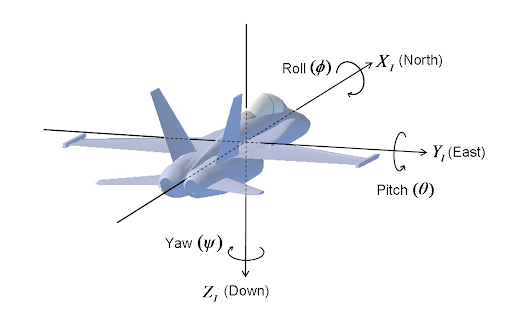
\includegraphics[scale=0.5]{./img/rpy.png}
\end{figure}
\url{https://youtu.be/pQ24NtnaLl8}

\subsubsection{Reprezentacja typu oś-kąt, dla macierzy {\bf R}, k-oś (musi być znormalizowana, czyli $\norm{k}=1$)}

Jak znaleźć oś z macierzy obrotu?

$tr \ R$ - Ślad macierzy {\bf R}

Suma elementów na przekątnej w macierzy {\bf R}:

\Large
$$
    tr \ R=1+2\cdot c_{\theta} \implies \theta=\arccos\left(\frac{tr \ R-1}{2}\right)
    \theta = \arccos\left(\frac{tr \ R - 1}{2}\right)
$$
\normalsize

Obrót w okół osi {\bf k} o kąt $\theta$:

\Large
$$
    \left[k\right]=\frac{R-R^{T}}{2\cdot\sin\theta}=
    \begin{bmatrix}
        0      & -k_{z} & k_{y}  \\[0.3em]
        k_{z}  & 0      & -k_{x} \\[0.3em]
        -k_{y} & k_{x}  & 0
    \end{bmatrix}
    \implies
    k =
    \begin{pmatrix}
        k_{x} \\
        k_{y} \\
        k_{z}
    \end{pmatrix}
$$
\normalsize

\newpage

Operacja odwrotna.
Mamy jakiś wektor {\bf k} i chcemy go unormować, żeby miał długość $1$ i mamy
podany kąt o jaki chcielibyśmy wykonać obrót:


Zwykły wektor $k_{zw}$, który chemy unormować do postaci $k =
    \begin{pmatrix}
        k_{x} \\
        k_{y} \\
        k_{z}
    \end{pmatrix}$, gdzie $\norm{k}=1$

Jakiej macierzy odpowiada obrót wokół wektora {\bf k} o kąt $\theta$?


\Large
$$
    rot(k, \theta ) = I_{3} + [-k] sin \theta + (1-cos \theta ) [k]^2
$$

$$
    rot(k, \theta)=
    \begin{bmatrix}
        \begin{array}{c|c|c}
            k_{x}^{2}(1-c_{\theta})+c_{\theta}       & k_{x}k_{y}(1-c_{\theta})-k_{z}s_{\theta} & k_{x}k_{z}(1-c_{\theta})-k_{y}s_{\theta} \\[0.3em]
            \hline
            k_{x}k_{y}(1-c_{\theta})+k_{z}s_{\theta} & k_{y}^{2}(1-c_{\theta})+c_{\theta}       & k_{y}k_{z}(1-c_{\theta})-k_{x}s_{\theta} \\[0.3em]
            \hline
            k_{x}k_{z}(1-c_{\theta})-k_{y}s_{\theta} & k_{y}k_{z}(1-c_{\theta})+k_{x}s_{\theta} & k_{z}^{2}(1-c_{\theta})+c_{\theta}
        \end{array}
    \end{bmatrix}
$$
\normalsize

\subsubsection{Obrót układ w okół dowolnego wektora (tutaj $v$) o kąt $\theta$}

Robimy to tak jakbyśmy byli we współrzędnych sferycznych. Na początku jest to rotacja w okół $Z$ o kąt $\alpha$

\Large
$$
    R\left(v, \varphi\right)=
    R(Z, \alpha)R(Y,\beta)R(Z, \varphi)R^{T}(Y, \beta)R^{T}(Z, \alpha)
$$
\normalsize


\begin{figure}[h!]
    \centering
    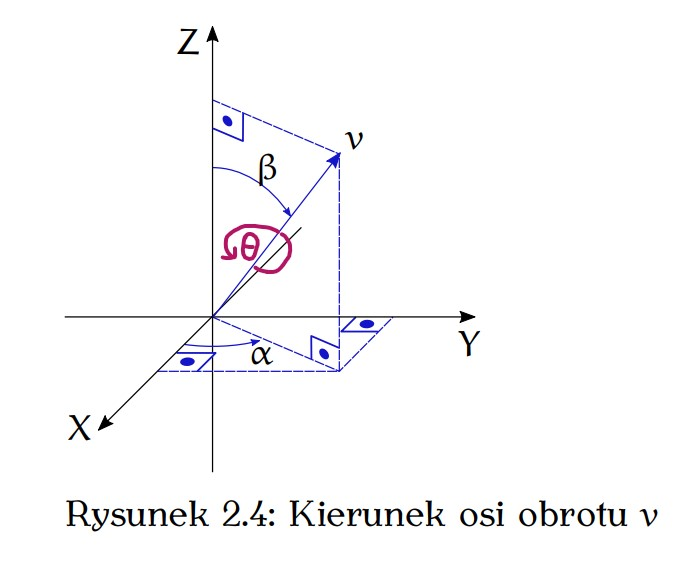
\includegraphics[scale=0.5]{img/kierunek_osi_obrotu.jpg}
\end{figure}

Ogólną macierz transformacji o dowolny (unormowany) wetkor można policzyć na wiele sposobów.
Jest to transformacja odwrotna do transformacji {\bf oś-kąt}

\newpage

\section{Wykład 3}

\subsection{Transformacje prędkości}

Zakładamy, że ruch polega wyłącznie na zmianie orientacji ciała (brak translacji), czyli:

\Large
$$
    c\left(t\right)=
    \begin{bmatrix}
        R(t)  & 0 \\[0.3em]
        0^{T} & 1
    \end{bmatrix}
    \cong
    R(t)
$$
\normalsize

Ponieważ $R(t)$ jest macierzą {\bf ortogonalną}, w każdej chwili zachodzi:

$$
    R(t)R^{T}(t)=R^{T}(t)R(t)=I_{3}
$$

skąd wynika:

$$
    \dot R(t)R^{T}(t)+R(t)\dot R^{T}(t)=\dot R^{T}(t)R(t)+R^{T}(t)\dot R(t)=0
$$

Otrzymujemy dwa pojęcia prędkości kątowej ciała sztywnego zdefniniowane macierzami:

\begin{enumerate}
    \item $\Omega_{S}=\dot R R^{T}$ - prędkość w {\bf przestrzeni} ({\bf S} od {\bf Space})
    \item $\Omega_{B}=R^{T} \dot R$ - prędkość w {\bf ciele} (definiowanie względem czegoś ruchomego) ({\bf B} od {\bf Body})
\end{enumerate}


Zachodzi:
\Large
$$
    \dot R =\Omega_{S}R=R\Omega_{B} \rightarrow \Omega_{S}=R\Omega_{B}R^{T}
$$
\normalsize
Obie macierze prędkości kątowej spełniają warunek:
\Large
$$
    \Omega+\Omega^{T}=0
$$
\normalsize
Macierz antysymetryczna/skośnie symetryczna:
\Large
$$
    \Omega = -\Omega^{T}
$$
\normalsize

Macierze $\Omega_{S}$ i $\Omega_{B}$ są skośnie symetryczne. Każda macierz skośnie symetryczna $3\times3$ jest zdefiniowana przez trzy parametry $\omega = \left(\omega_{1}, \omega_{2}, \omega_{3}\right)^{T}$:
\Large
$$
    \Omega=\left[\omega\right]=
    \begin{bmatrix}
        0           & -\omega_{3} & \omega_{2}  \\[0.3em]
        \omega_{3}  & 0           & -\omega_{1} \\[0.3em]
        -\omega_{2} & \omega_{1}  & 0
    \end{bmatrix}
$$
\normalsize
Rozmieszczenie składowych wektora $\omega$ w macierzy $\left[\omega\right]$ jest takie żeby (gdzie $v$ to wektor w 3D):

\Large
$$
    \Omega v = \omega \times v
$$
\normalsize

\newpage

Stosując to rozumowania możemy zdefiniować:

\begin{itemize}
    \item $\Omega_{S} = \left[\omega_{S}\right]$ - wektor prędkości kątowych względem układu nieruchomego w przestrzeni
    \item $\Omega_{B} = \left[\omega_{B}\right]$ - wektor prędkości kątowych względem układu ciała
\end{itemize}

Ponieważ obrót był pierwotnie opisany w macierzy $4\times4$ tak też robimy:

$$
    \begin{bmatrix}
        \Omega & 0 \\[0.3em]
        0^{T}  & 0 \\[0.3em]
    \end{bmatrix}
$$

gdzie $\Omega$ to byle które z prędkości.



Rozważmy teraz przykład ogólny ruchu zawierającego zarówno przesunięcie (translacje), jak i obrót:

$$
    c(t)=
    \begin{bmatrix}
        R(t)  & T(t) \\[0.3em]
        0^{T} & 1    \\[0.3em]
    \end{bmatrix}
$$

Zróżniczkowane po czasie:


$$
    \dot c(t)=
    \begin{bmatrix}
        \dot R(t) & \dot T(t) \\[0.3em]
        0         & 0         \\[0.3em]
    \end{bmatrix}
$$



Macierz przedstawiająca prędkości względem przestrzeni

$$
    V_{S} = \dot c c^{-1}
$$



Macierz przedstawiająca prędkości względem ciała

$$
    V_{B} = c^{-1} \dot c
$$

Na mocy powyższych defnicji otrzymujemy:

$$
    V_{S}=
    \begin{bmatrix}
        \dot R & \dot T \\[0.3em]
        0^{T}  & 0      \\[0.3em]
    \end{bmatrix}
    \begin{bmatrix}
        R_{T} & -R^{T}T \\[0.3em]
        0^{T} & 1       \\[0.3em]
    \end{bmatrix}
$$


tzn.
\Large
$$
    V_{S}=
    \begin{bmatrix}
        \Omega_{S} & \dot T-\Omega_{S}T \\[0.3em]
        0^{T}      & 0
    \end{bmatrix}
    \cong
    v_{S}
    =
    \begin{pmatrix}
        \dot T-\omega_{S}\times T \\[0.3em]
        \omega_{S}
    \end{pmatrix}
    =
    \begin{pmatrix}
        \dot T + \left[T\right]\omega_{S} \\[0.3em]
        \omega_{S}
    \end{pmatrix}
$$
\normalsize
\newpage

Wektor $v_{S} \in \mathbb{R}^{6}$ reprezentujący macierz $V_{S}$ nazywany {\bf skrętnikiem w przestrzeni}. W podobny sposób wyznaczamy $V_{B}$:

$$
    V_{B}=
    \begin{bmatrix}
        R^{T}\dot R & R^{T}\dot T \\[0.3em]
        0^{T}       & 0           \\[0.3em]
    \end{bmatrix}
    \cong
    v_{B}
    =
    \begin{pmatrix}
        R^{T}\dot T \\[0.3em]
        \omega_{B}
    \end{pmatrix}
$$

Korzystając z własności prędkości kątowych w przestrzeni i w ciele oraz z izomofrizmu $\left[ \ \right]$ otrzymujemy następujący związek między skrętnikami:

$$
    v_{S}=
    \begin{bmatrix}
        R     & \left[T\right]R \\[0.3em]
        0^{T} & R
    \end{bmatrix}
    v_{B}
$$



Interpretacja macierzowych prędkości $V_{S}$ i $V_{B}$. Niech będzie danny punkt P w układzie ciała, o współrzędnych $p \in \mathbb{R}$. Jego współrzędne układu przestrzeni:

$$
    s=Rp+T
$$

Obliczamy prędkość $\dot s=\dot R p + T$, co po podstawieniu $p=R^{T}\left(s-T\right)$ prowadzi do wzoru:

$$
    \dot s = \dot R R^{T} (s-T)+\dot T= \omega_{S}\times (s-T)+\dot T
$$

Ostatnią zależność można zapisać jako:

$$
    \begin{pmatrix}
        \dot s \\[0.3em]
        0
    \end{pmatrix}
    =V_{S}
    \begin{pmatrix}
        s \\[0.3em]
        1
    \end{pmatrix}
$$

Wynika stąd, że macierzowa prędkość $V_{S}$ określa prędkość ruchu punktu P o współrzędnych jednorodnych $(p^{T}, 1)^{T}$, względem układu przestrzeni. Prowadz to do wniosku:

$$
    \begin{pmatrix}
        R^{T}\dot s \\[0.3em]
        0
    \end{pmatrix}
    =V_{B}
    \begin{pmatrix}
        p \\[0.3em]
        1
    \end{pmatrix}
$$


\newpage

\section{Wykład 4}

\subsection{Kinematyka i algorytm Denavita-Hartenberga}

Liczenie kinematyki manipulatora.

Chcemy opisać położenie i orientacje ostatniego ogniwa w manipulatorze, które nazywa się chwytakiem (end-effector), ostatni układ współrzednych to jest układ efektora. Mamy też zerowy układ współrzednych (ten nieruchomy) względem, którego wszystko chcemy przeliczać. Zwykle jest to jakiś punkt, który gdzieś się znajduje np. jakaś platforma. Układ zerowy nosi nazwę układu "podstawowego" lub "bazowego" nalezy go traktować jako układ przestrzeni.

Opis położenia końcówki ramienia manupulatora, który np przykręca śróbkę. Musi być w obeć sróbki pod dobrym kontem itp. W związku z tym naszym celem jest zorientowanie się gdzie znajduje się koncówka manipulatora, jaką ma orientację i czy jest ona dobra.
Tak więc musimy wyrazić położenie końcówki względem układu podstawowego. Uzyskanie takiej transofrmacji nazywa się "kinematyką".
Taką kinematykę wylicza się względem algorytmu {\bf Danovita-Hartenberga}.


Za pomocą $4$ parametrów chcemy opisać ruch jednego układu współrzednych względem drugiego układu współrzednych.

% 1:15:00

\newpage

Manipulator sztywny definiujemy jako układ złożony z pewnej liczby
ciał sztywnych (ramion, ogniw) połączonych przegubami. Przyjmujemy,
że przeguby są typu obrotowego lub typu przesuwnego; bardziej złożone
przeguby można traktować jako kombinację tych dwóch typów. Ramiona manipulatora tworzą tzw. łańcuch kinematyczny. Początkiem łańcucha jest nieruchoma podstawa, a końcem – efektor manipulatora. Będziemy zakładać, że łańcuch kinematyczny jest otwarty, tzn. efektor nie
pokrywa się z podstawą manipulatora. Taki manipulator nazywamy szeregowym. Liczbę przegubów manipulatora nazywamy jego liczbą stopni
swobody. Jeśli jeden przegub może wykonywać dwa niezależne ruchy to każdy z nich jest niezależną liczbą stopni swobody. Schematyczny widok manipulatora szeregowego przedstawia rysunek poniżej. Na Rysunku symbole $L_{1}, L_{2}, \dots , L_{n}$ oznaczają kolejne ogniwa manipulatora.


\begin{figure}[h!]
    \centering
    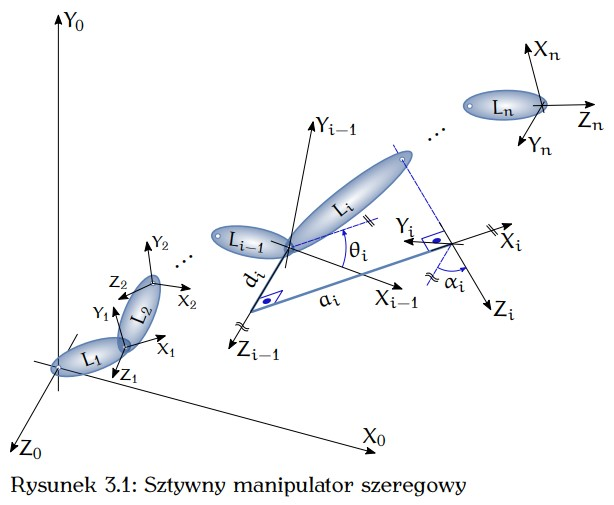
\includegraphics[scale=0.5]{img/manipulator_sz.jpg}
\end{figure}

Z reguły opisując manipulator nadajemy im nazwy związane z ilościa stopni swobody.
Np podwójne wachadło (RR) oznacza, że są 2 obrotowe stopnie swobody, manipulator RTR to obrotowy, przesuwny i obrotowy itp. itd..

Przez przestrzeń przegubową manipulatora rozumiemy wektor. Każda składowa tego wektora to jest położenie pojedyńczego przegubu. Czyli np manipulator o 3 stopniach swobody bedzie miał przestrzeń przegubową $q_{1}, q_{2}, q_{3}$.

Jeśli chcemy opisać kinematykę, czyli położenie i orientację punktu pracy/efektora względem podstawy. Wybieramy dwa specjalne układy współrzedne.
Pierwszy układ współrzednych związany jest z podstawą, jest to układ "bazowy", "podstawowy", jest nieruchomy (układ przestrzeni)(Space).
Drugi układ związany jest z efektorem, jest to układ ciała (Body).
Chcemy za ich pomocą wyrazić kinematykę manipulatora czyli powiedzieć gdzie znajduje się efektor względem układu podstawowego i jak jest względem niego skierowany.

\newpage

\subsection{Algorytm Denavita-Hartenberga}

% 3:40 wyk4
\begin{enumerate}
\item Przyjmujemy oś $Z_i$ tak, by ruch w przegubie następnym przegubie ($i+1$) zachodził względem niej;
\item Prowadziny normalną do osi $Z_{i-1}$ i $Z_i$;
\item Początek układu $i$ umieszczany na przecięciu normalnej z osią $Z_i$;
\item oś $X$ prowadzimy wzdłuż normalnej, oś $Y_i$ spełnia warunek $X_u \times Y_i = Z_i$
\item (a oś $Y$, nie jest nam potrzebna)
\begin{enumerate}
    \item Jeśli koeljne osie $Z$ są równoległe (nieskończenie wiele normalnych),
    to wybieramy przechodzącą przez początek układu $i-1$
    \item jeśli $Z_{i-1} = Z_i$, to postępujemy "zgodnie ze zdrowym rozsądkiem"
\end{enumerate}
\end{enumerate}

\Large
$$
    A_{i-1}^i (q_i) = Rot(Z,q_i) \cdot Trans(Z,d_1) \cdot Trans( X, a_i ) \cdot Rot( X, \alpha_i )
$$
\normalsize

\begin{table}[h!]
    \centering
    \Large
    \begin{tabular}{c|c|c|c|c}
            & $\theta_i$& $d_i$     & $a_i$     & $\alpha_i$\\ \hline
        1   &           &           &           &           \\ \hline
        2   &           &           &           &           \\ \hline
        3   &           &           &           &           \\
    \end{tabular}
\end{table}


\section{Kinematyka}

Współrzedne efektora:
$$
    y(t) = k( q(t) )
$$

Prędkość ruchu efektora. $J(q)$ - jest jakobianem analitycznym:
$$
    \dot{y}(t) = J(q) \dot{q}
    \ \ \ \
    J(q) = \frac{\delta k}{\delta q}
$$

\subsection{Macierz kinematyki}
\Large
$$
    K \in \textbf{R}^6, \ \
    K = \begin{bmatrix}
        x_{ch} \\
        y_{ch} \\
        z_{ch} \\
        \phi \\
        \theta \\
        \xi
    \end{bmatrix}
$$
\normalsize

Pierwsze 3 elementy $K$ określają współrzędne kartezjańskiego, drugie 3 współrzene obrotowe.

\subsection{Jakobian}
\Large
$$
    J(q)_{m\times n} = \begin{bmatrix}
        \frac{\delta k_1}{\delta q} \\
        \frac{\delta k_2}{\delta q} \\
        ... \\
        \frac{\delta k_m}{\delta q}
    \end{bmatrix}
    = \begin{bmatrix}
        \frac{\delta k_1}{\delta q_1} &
        \frac{\delta k_1}{\delta q_2} &
        ... &
        \frac{\delta k_1}{\delta q_n} \\
        \vdots \\
        \vdots \\
        \frac{\delta k_m}{\delta q_1} &
        \frac{\delta k_m}{\delta q_2} &
        ... &
        \frac{\delta k_m}{\delta q_n}
    \end{bmatrix}
$$
\normalsize

% praca wirtualna wykład 11-04, 32:00
\subsubsection{Zasada Pracy Wirtualnej}
(Wymiennie z "Zasadą Mocy Wirtualnej")

$$  \tau^T\ dy = f^T dq                 \hspace{1cm}
    \tau^T\ \dot{y} = f^T \dot{q}       \hspace{1cm}
    \tau^T J \dot{q} = f^T \dot{q}      \hspace{1cm}
$$

\Large
$$ f = \tau J^T $$
\normalsize

\begin{kol2}
    Praca w przestrzeni zewnętrznej
    $$ \tau^T\ dy $$
    $\tau$ - siły (/momenty sił) wywiarne na chwytak
\end{kol2}
\begin{kol2}
    Praca w przestrzeni przegubowej
    $$ f^t\ dq$$
    $f$ - siły (/momenty sił) wywiarne w przegubach
\end{kol2}

% praca wirtualna wykład 11-04, 54:00
\subsubsection{Konfiguracje osobliwe i regularne}

$$ rank\{J\} \leq min\{ m, n \} $$

\begin{enumerate}
    \item Konfiguracja regularna - jakobian nie traci rzędu
    \item Konfiguracja osobliwa - jakobian traci rząd wierszowy.

    Wierszowy, bo to znaczy, że pewna współrzędna w tej konfiguracji nie wpływa na położenie chwytaka.

    \begin{enumerate}
        \item $m > n$ - wszystkie konfiguracje są osobliwe;
        \item $m = n$ - osobliwa, tylko i tylko w tedy, gdy $ det{J} = 0$;
        \item $m < n$ (przypadek redundantny) osobliwość,
        gdy wszystkie minory stopnia $m$ są równe $0$ ("największe możliwe minory").
    \end{enumerate}

\end{enumerate}

\newpage

\section{Przydatne wzorki}
\subsection{Trygonometria}

\begin{kol2}

    \noindent
    Suma kątów

    $$  \sin{\alpha}\pm\sin{\beta}=
        2\sin{\frac{\left(\alpha\pm\beta\right)}{2}}
        \cos{\frac{\left(\alpha\mp\beta\right)}{2}} $$
    $$  \cos{\alpha}+\cos{\beta}=
        2\cos{\frac{\left(\alpha+\beta\right)}{2}}
        \cos{\frac{\left(\alpha-\beta\right)}{2}} $$
\end{kol2}
\begin{kol2}

    \noindent
    Wartości funckji
    $$
        \begin{array}{c|c|c|c|c|c|c}
            & 0^\circ   & 30^\circ      & 45^\circ      & 60^\circ      & 90^\circ  & 180^\circ  \\
            & 0         & \frac\pi6     & \frac\pi4     & \frac{\pi}3   & \frac\pi2 & \frac\pi2  \\ \hline
        sin & 0         & \frac12       & \frac{\sqrt2}2&\frac{\sqrt3}2 & 1         & 0  \\
        cos & 1         & \frac{\sqrt2}2& \frac{\sqrt2}2& \frac12       & 0         & -1 \\ \hline
        tg  & 0         & \frac{\sqrt3}3& 1             & \sqrt3        & -         & 0  \\
        ctg & -         & \sqrt3        & 1             & \frac{\sqrt3}3& 1         & -  \\
        \end{array}
    $$
\end{kol2}

\vspace{0.5cm}
\begin{kol2}

    \noindent
    Funkcje sumy kątów lub ich wielokrotności

    $$  sin( x\pm y) = sin(x)cos(y) \pm cos(x)sin(y) $$
    $$  cos( x\pm y) = cos(x)cos(y) \mp sin(x)sin(y) $$
    $$  sin(2x) = 2sin(x)cos(x) $$
    $$  cos(2x) = sin^2x - cos^2x   $$

\end{kol2}
\begin{kol2}

    \noindent
    Wzory redukcyjne

    \centering
    \begin{tabular}{c c}
        Parzystość f.       & Nieparzystość f. \\ \hline
        $cos(x) = cos(-x)$  & $sin(-x) = - sin(x)$ \\
                            & $tg(-x) = -tg(x)$ \\
                            & $ctg(-x) = - ctg(x)$ \\
    \end{tabular}

    $$  sin( x \pm \frac{\pi}{2} ) = \pm cos( x ) $$
    $$  cos( x \pm \frac{\pi}{2} ) = \mp sin( x ) $$
\end{kol2}

\end{document}